\section{Contratos inteligentes}
\subsection{Fundamentos}

\begin{frame}{Contratos inteligentes}
    \begin{itemize}
        \item 1997: Primeira proposta;
        \item 2014: Primeira aplicação - blockchain Ethereum;
        \item Outras plataformas que implementam CIs: Hyperledger Fabric, Corda e Stellar.
    \end{itemize}
    \begin{block}{Desenvolvimento de um CI}
    Cláusulas contratuais estabelecidas em comum acordo entre as partes envolvidas são expressas por meio de programas de computador executáveis.
    \end{block}
    \begin{itemize}
        \item Solidity: linguagem desenvolvida para CIs na Ethereum;
        \item CIs são sempre compilados para \textit{bytecode};
        \item O \textit{bytecode} é executado na MVE.
    \end{itemize}
\end{frame}

\begin{frame}{Contratos inteligentes}
    \begin{figure}[!htb]
     \centering
     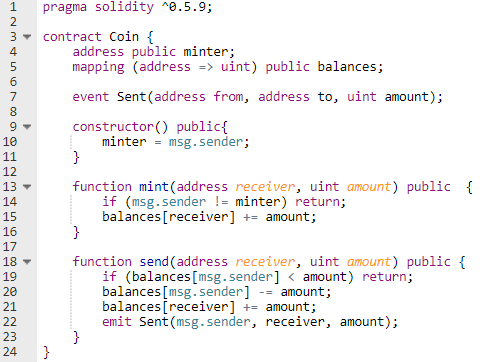
\includegraphics[scale=0.6]{figuras/contratos-inteligentes/exemplo_codigo_solidity.png}
    \end{figure}
\end{frame}

\begin{frame}{Contratos inteligentes}
    \begin{block}{}
    A utilização dos CIs possui um ciclo de vida de quatro fases: \textbf{criação}; \textbf{implantação}; \textbf{execução}; e \textbf{conclusão}.
    \end{block}
    \begin{figure}[!htb]
        \centering
        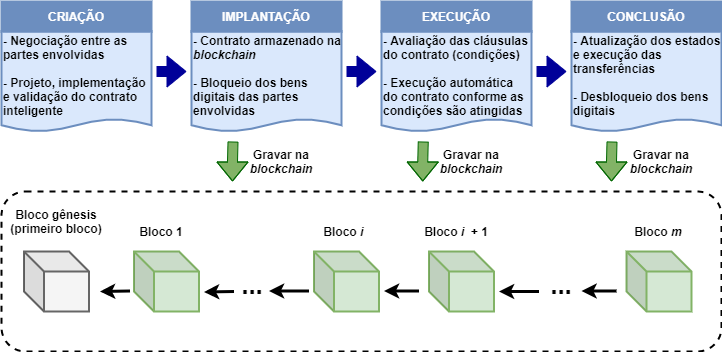
\includegraphics[scale=0.4]{figuras/contratos-inteligentes/contrato_ciclo_de_vida.png}
    \end{figure}    
\end{frame}

\subsection{Vulnerabilidades e ataques}

\begin{frame}{Contratos inteligentes}
    \begin{block}{}
    Devido à \textbf{imutabilidade} da blockchain, um contrato implementado não pode mais ser alterado.
    \end{block}
    \begin{block}{}
    Esta propriedade agrega \textbf{integridade} à tecnologia blockchain, mas também ressalta a importância da implementação de contratos livres de erros e de acordo com boas práticas.
    \end{block}
    \begin{alertblock}{}
    \textbf{Vulnerabilidades} deixadas nos códigos dos CIs podem torná-los alvos de \textbf{ataques}.
    \end{alertblock}
\end{frame}

\begin{frame}{Contratos inteligentes - Vulnerabilidades e ataques}
    \begin{block}{}
    Aplicações desenvolvidas por meio de CIs costumam envolver transferências e gerenciamento de grandes quantidades de bens digitais.
    \end{block}
    \begin{itemize}
        \item Primeiro ataque: \textit{The DAO Attack} (2016);]
        \item Vulnerabilidade explorada: \textbf{Reentrância};
        \item Um usuário malicioso transferiu \textbf{3,6 milhões} em Ether para sua conta;
        \item Equivalente a \textbf{50 milhões} de dólares.
    \end{itemize}
    \begin{block}{}
    Este caso teve grande repercussão e motivou estudos e estratégias para \textbf{detecção} e \textbf{prevenção} de \textbf{vulnerabilidades} em CIs. 
    \end{block}
\end{frame}

\begin{frame}{Contratos inteligentes - Vulnerabilidades e ataques}
    \begin{block}{}
    Parte dos erros e vulnerabilidades explorados em ataques contra os CIs são ocasionados pelo desalinhamento que há entre a semântica da linguagem Solidity e a intuição dos desenvolvedores.
    \end{block}
    \begin{block}{}
    Solidity possui elementos similares ao de outras linguagens, mas que não são implementados da mesma forma.
    \end{block}
    \begin{exampleblock}{}
    Há registro de uma série de vulnerabilidades que resultaram na exploração de CIs e enormes perdas financeiras.
    \end{exampleblock}
\end{frame}

\begin{frame}{Contratos inteligentes - Vulnerabilidades e ataques}
    Vulnerabilidades alvos desta pesquisa:
    \begin{itemize}
        \item Reentrância;
        \item \textit{Delegatecall injection};
        \item Contrato suicida.
    \end{itemize}
\end{frame}

\begin{frame}{Vulnerabilidade - Reentrância}
    \begin{itemize}
        \item Explorada no \textit{The DAO Attack};
        \item Pode ocorrer quando um contrato pode ser invocado recursivamente sucessivas vezes;
        \item Ocorre por meio de uma função \textit{callback}.
    \end{itemize}
    \begin{figure}[!htb]
        \centering
        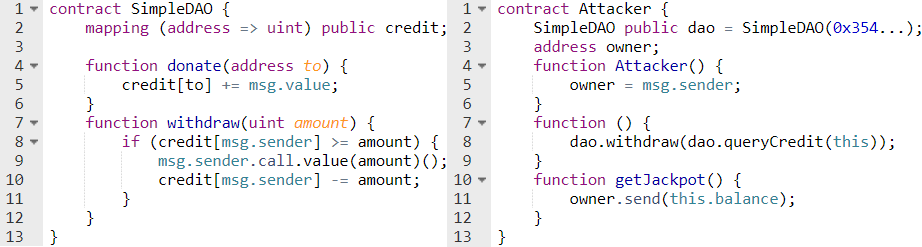
\includegraphics[scale=0.45]{figuras/contratos-inteligentes/reentrancia-exemplo.png}
    \end{figure}
\end{frame}

\begin{frame}{Exploração da reentrância}
    \begin{itemize}
        \item 1º Passo: Publicação do contrato.
    \end{itemize}
    \begin{figure}[!htb]
     \centering
     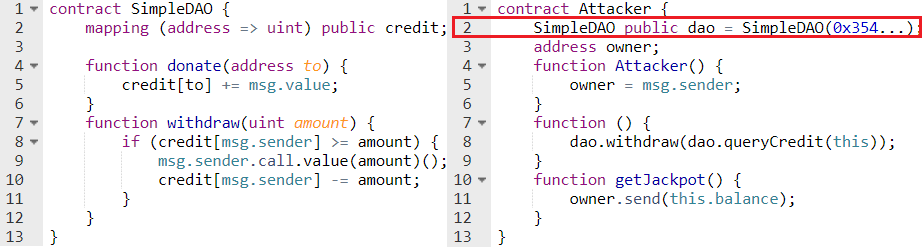
\includegraphics[scale=0.45]{figuras/contratos-inteligentes/reentrancia-passo-1.png}
    \end{figure}    
\end{frame}

\begin{frame}{Exploração da reentrância}
    \begin{itemize}
        \item 2º Passo: Doação para o contrato utilizando sua CPE.
    \end{itemize}
    \begin{figure}[!htb]
     \centering
     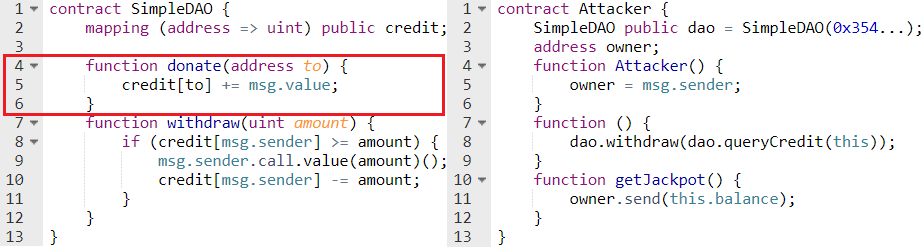
\includegraphics[scale=0.45]{figuras/contratos-inteligentes/reentrancia-passo-2.png}
    \end{figure}     
\end{frame}

\begin{frame}{Exploração da reentrância}
    \begin{itemize}
        \item 3º Passo: Invocação da função \textit{fallback}, que invoca a função \texttt{withdraw};
        \item Ether é transferido para o \texttt{Attacker}.
    \end{itemize}
    \begin{figure}[!htb]
     \centering
     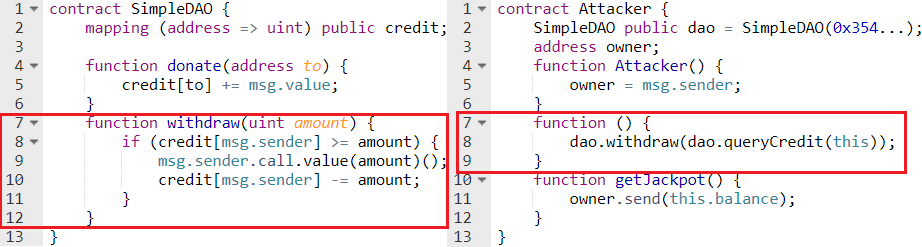
\includegraphics[scale=0.45]{figuras/contratos-inteligentes/reentrancia-passo-3.png}
    \end{figure}     
\end{frame}

\begin{frame}{Exploração da reentrância}
    \begin{itemize}
        \item 4º Passo: Chamadas sucessivas à função \texttt{withdraw}.
        \item Da forma como é usada, a função \texttt{call}, que é uma função \textit{callback}, permite nova invocação da função \texttt{withdraw} antes da execução do comando \texttt{credit[msg.sender] -= amount};
        \item Verificação da linha 8 tem êxito novamente.
    \end{itemize}
    \begin{figure}[!htb]
     \centering
     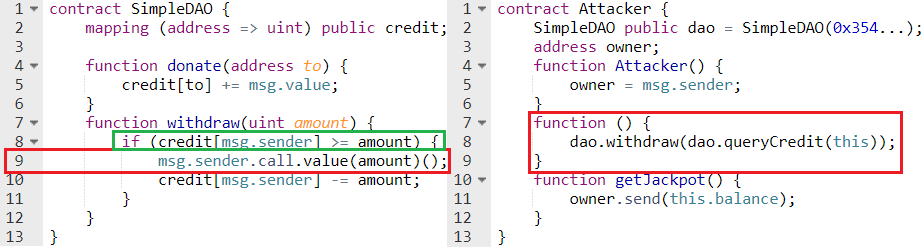
\includegraphics[scale=0.45]{figuras/contratos-inteligentes/reentrancia-passo-4.png}
    \end{figure}     
\end{frame}

\begin{frame}{Exploração da reentrância}
    \begin{itemize}
        \item As transferências são realizadas sucessivamente até ocorrer um dos seguintes eventos:
        \begin{itemize}
            \item Todo \textit{gas} é utilizado;
            \item Pilha de chamadas da MVE é totalmente preenchida;
            \item Saldo do \texttt{SimpleDAO} é zerado.
        \end{itemize}
        \item Como evitar:
        \begin{itemize}
            \item Atualizar as variáveis de estado antes da invocação de outro contrato;
            \item Trava \textit{mutex};
            \item Utilizar o método \texttt{transfer}.
        \end{itemize}
    \end{itemize}
    \begin{block}{}
    Os danos causados pelo \textit{The DAO Attack} foram revertidos por meio de um \textit{hard fork}, que causou uma divisão dos mineradores da Ethereum.
    \end{block}
\end{frame}

\begin{frame}{Vulnerabilidade - \textit{Delegatecall injection}}
    \begin{itemize}
        \item Explorado no ataque contra a \textit{Parity Multsignature Wallet};
        \item Em 2017, 31 milhões de dólares foram subtraídos em um ataque;
        \item \texttt{delegatecall}: Usado para inserir o \textit{bytecode} de um contrato no \textit{bytecode de outro contrato};
        \item O contrato que é chamado pode alterar as variáveis de estado do contrato que o invocou.
    \end{itemize}
\end{frame}

\begin{frame}{Exploração da \textit{delegatecall injection}}
    \begin{figure}[!htb]
     \centering
     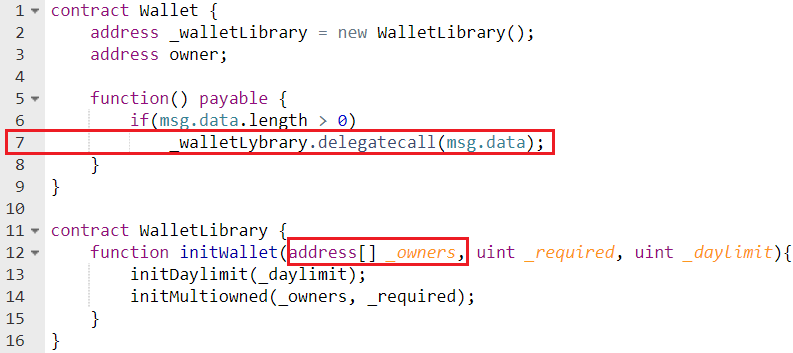
\includegraphics[scale=0.5]{figuras/contratos-inteligentes/delegatecall-passo1.png}
    \end{figure}    
\end{frame}

\begin{frame}{Exploração da \textit{delegatecall injection}}
    \begin{itemize}
        \item Envio de uma transação com o campo \texttt{msg.data} contendo \texttt{initWallet} como a função a ser chamada;
        \item Os endereços de posse do contrato (\texttt{\_owners}) foram substituídos pelo endereço do atacante;
        \item Foi realizada a transferência de 31 milhões de dólares em Ether.
        \item Como evitar: 
        \begin{itemize}
            \item Declarar contrato a ser compartilhado (\texttt{WalletLibrary}) como uma biblioteca (\texttt{library}).
        \end{itemize}
    \end{itemize}
\end{frame}

\begin{frame}{Vulnerabilidade - Contrato suicida}
    \begin{itemize}
        \item Um contrato pode ser ``morto'' pelo dono do contrato ou outra parte confiável;
        \item Métodos: \texttt{suicide} ou \texttt{selfdestruct};
        \item O \textit{bytecode} e o armazenamento do contrato é deletado;
        \begin{block}{}
        A vulnerabilidade \textbf{contrato suicida}, acontece quando uma \textbf{autenticação inadequada} permite que algum invasor tome posse do contrato e execute a função para matar o contrato.
        \end{block}
        \item Foi explorada em um segundo ataque contra \textit{Parity Wallet};
        \item \textbf{280 milhões} de dólares em Ether foram permanentemente \textbf{bloqueados}.
    \end{itemize}
\end{frame}

\begin{frame}{Exploração da vulnerabilidade contrato suicida}
    \begin{itemize}
        \item Como resposta ao primeiro ataque, foi adicionado o modificador \texttt{only\_uninitialized};
        \item Porém, o contrato \texttt{WalletLibrary} foi deixado como não inicializado;
        \item O invasor passou pelo modificador, se declarou dono do contrato, e invicou o método suicide.
    \end{itemize}
    \begin{figure}[!htb]
     \centering
     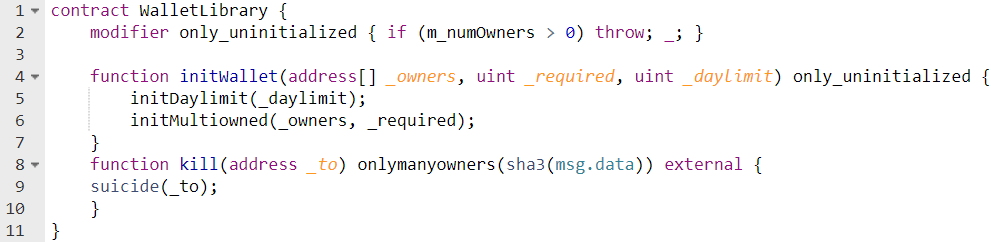
\includegraphics[scale=0.4]{figuras/contratos-inteligentes/parity-corrigido.png}
    \end{figure}    
\end{frame}

\begin{frame}{Ethereum - Vulnerabilidades}
    \begin{block}{}
    Além da reentrância, \textit{delegatecall injection} e contrato suicida, existem diversas outras vulnerabilidades encontradas na literatura, e que devem ser evitadas.
    \end{block}
    \begin{block}{}
    Desde o \textit{The DAO Attack}, muitos esforços foram realizados para desenvolvimento de métodos, ferramentas e frameworks para \textbf{verificação de CIs} e \textbf{detecção de vulnerabilidades}.
    \end{block}
\end{frame}